\section{\texorpdfstring{Pokročilejší vyčíslitelnost}{Pokročilejší vyčíslitelnost}}
\vspace{5mm}
\large

\subsection{R.S. množiny}

\begin{definition}[Postův problém podruhe]
	\[ \exists A: \emptyset <_T A <_T \emptyset^{\prime} \]

	Byl vyřešen nezávislé Friedberg-Mučník pomoci tzv. prioritních metod.
	\begin{enumerate}
		\item finite injury $\emptyset^{\prime}$-priority
		\item infinite injury $\emptyset^{\prime\prime}$
		\item $\emptyset^{\prime\prime}$-priority
	\end{enumerate}
\end{definition}

\subsection{Forcing}

\begin{definition}[Cantor space]
	Hlavní myšlenka je použit tzv \href{https://en.wikipedia.org/wiki/Cantor_space}{Cantorův prostor} $2^{\omega}$.
	Což je prostor všech zobrazení
	\[ f:\N \to \{ 0, 1 \} \]

	Je úplný metrický prostor.
\end{definition}

\begin{note}
	Okolí v Cantorovém prostoru je
	\[ o_{\sigma} = \{ B: \sigma \prec B \} \]
	Pak vzdálenost
	\[ \rho(\ldots) \leq 2^{-\sigma} \]
\end{note}

\begin{definition}[Finite extension method (Cohen)]
	Souvisí s Cohenovým forcingem v teorii množin kterým vyřešil hypotézu continua.
\end{definition}

\begin{theorem}[Bairová věta o kategoriích]
	Máme úplný metrický prostor. Pak
	\[ \bigcap_{\text{spočetná}} (\text{otevřené, husté}) \ne \emptyset \]

	Jde o ekvivalentní formulace. Viz \href{https://en.wikipedia.org/wiki/Baire_category_theorem}{Baire category theorem}.
\end{theorem}
\begin{proof}
	Hint:

	Nechť první bod je $A_0$ leží v otevřené husté množině.
	Jelikož je otevřená, existuje okolí $A_0$ které je uvnitř množiny.
	Z hustoty v tomto okolí je další bod, je taky s okolím atd.

	Takovým postupem vytvoříme Cauchy posloupnost, která kvůli úplnosti má limitu.
	Tato limita leží v průniku.

	Speciálně platí v Cantorovém prostoru.

	% obrazek, 11. lekce 36:00
	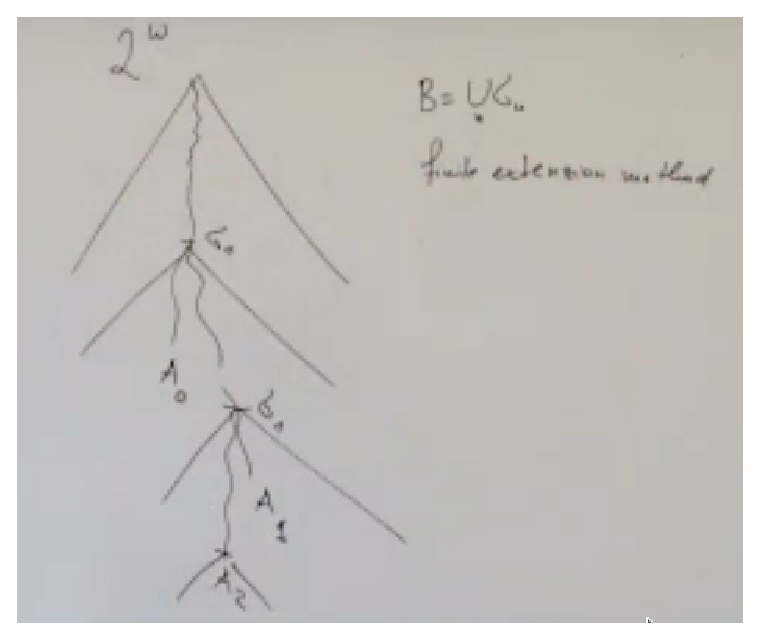
\includegraphics[scale=0.4]{baire_c.eps}
\end{proof}

\begin{definition}[1-generická]
	A je 1-generická když
	\[ \forall e \exists \sigma(\sigma \prec A \land (\Phi_e(\sigma)(e)\downarrow \lor (\forall \tau \geq \sigma: \Phi_e(\tau)(e)\uparrow)) \]
	Buď s nějakým začátkem konverguje, nebo tzv. silně diverguje (i v okolí).

	První podmínka je ekvivalentní
	\[ \forall \sigma \prec B: \Phi_e(B)(e) \downarrow \]

	Druhá je ekvivalentní
	\[ \forall \sigma \prec B: \Phi_e(B)(e) \uparrow \]
\end{definition}

\begin{theorem}[Existence 1-generické]
	Existuje 1-generická:
	\[ A \leq_T \emptyset^{\prime} \]
\end{theorem}
\begin{proof}
	Používá se finite extension method.

	Pomoci $\emptyset^{\prime}$ vytvoříme $\emptyset^{\prime}$-posloupnost $\{\sigma_n\}_n$:
	\[ \sigma_{n + 1} \preccurlyeq \sigma_n \]

	Pak
	\[ A = \bigcup \sigma_n \]

	BUNO: $\sigma_0 = \emptyset$.
	Indukční krok: máme $\sigma_n$ chceme další.
	Zkusíme:
	%todo změna indexu z n na e
	\[ \exists \sigma_e \preccurlyeq \tau: (\Phi_e(\tau)(e)\downarrow) \]
	Pokud ano, vezmeme první takové a $\sigma_{e + 1} = \tau$.
	Jinak $\sigma_{e + 1} = \sigma_e$.

	Otázka je 1-kvantifikatorová neboli $\leq_T \emptyset^{\prime}$. Neboli $\emptyset^{\prime}$ umí rozhodnout.
\end{proof}

\begin{theorem}[Kleene-Post]
	Existuji nerekurzívní $A, B \leq_T \emptyset^{\prime}$ takové, že $A, B$ jsou $T$-neporovnatelné.
\end{theorem}
\begin{proof}
	Pomoci $\emptyset^{\prime}$ vytvoříme monotonní $\emptyset^{\prime}$-posloupnosti:
	\[ A = \bigcup \{\alpha_n\}_n, B = \bigcup \{\beta\}_n \]

	BUNO: $\alpha_0 = \beta_0 = \emptyset$.

	Indukční krok: 2 podkroky, protože potřebujeme zajistit
	\[ (A \nleq_T B \simeq \Phi_e(B) \neq A) \land (B \nleq_T A \simeq \Phi_e(A) \neq B) \]
	Stačí jedná z podmínek, druhá symetricky.

	Otázka
	\[ \exists \beta_e \preccurlyeq \tau: (\Phi_e(\tau)(x_0)\downarrow = 0) \]
	kde $x_0 = |\alpha_e|$, $\alpha_e(x_0)$ není definované.

	Pokud ANO, tak
	\[ \alpha_{e + 1} = \alpha_e + 1, \beta_{e + 1} = \tau \]
	S tím, že $\tau$ první které padlo.
	Pak pro libovolnou $\beta_{e + 1} \preccurlyeq B$ platí
	\[ \Phi_e(B)(x_0) = 0 \land A(x_0) = 1 (A \preccurlyeq \alpha_{e + 1})\]

	Jinak
	\[ \alpha_{e + 1} = \alpha_e + 0, \beta_{e + 1} = \beta_e \]
	Pak
	\[ A(x_0) = 0 \land (B(x_0) \downarrow = 1 \lor B(x_0) \uparrow) \]
\end{proof}

\begin{theorem}[R.S. a 1-generické]
	Žádná rekurzívní není 1-generická.
\end{theorem}
\begin{proof}
	A je rekurzívní, najdeme $e_0$ takové, že
	\[ \Phi_{e_0}(A)(e_0) \uparrow \land \forall B \neq A: \Phi_{e_0}(B)(e_0) \downarrow \]

	\[ \mu_y (B(y) \neq A(y)) \]

	Pak máme divergenci v množině A ale nikoliv silnou (v okolí konverguje).
\end{proof}

\begin{note}
	Těch A, které nejsou 1-generické je málo.
	Přesněji v topologickém smyslu (2 kategorie) 1-generická jsou "všude".

	Odbočka, pro funkcionál $dom(\Phi_e)$ je otevřená.
	Doplněk je dle definice uzavřená, vnitřek je největší otevřená, takže je ok.
	Zbývá hranice, a takových je málo.
\end{note}

\begin{definition}[n-generická]
	Podobně jako 1-generická, ale místo $\Sigma_1^0$ vezmeme $\Sigma_n^0$.
\end{definition}

\begin{note}
	Problém prioritních metod.
	% todo prednaska 11, od 1:16:00
\end{note}

\begin{theorem}[Low]
	A je 1-generická a $A \leq_T \emptyset^{\prime} \Rightarrow A$ je tzv. low.
	\[ A^{\prime} \equiv_T \emptyset^{\prime} \]

	Libovolný skok \cref{jump} je $\emptyset^{\prime}$.
\end{theorem}
\begin{proof}
	% todo prednaska 12, od 1:07:00
\end{proof}

\subsection{Algoritmická náhodnost}

\subsection{Kolmogorovská složitost, Martingale}
